\documentclass[a4paper]{article}

\usepackage[utf8]{inputenc}
\usepackage{graphicx}
\usepackage{subfig}

\usepackage{makeidx}  % allows for indexgeneration

\begin{document}


\title{DH2323: Lab 1}
\author{Karl Johan Andreasson \and Erik Fahlén}

\maketitle
\clearpage

\section{Methods}
Because we both initially thought that this lab seemed to be quite simple, we ended up doing two separate approaches and then looking at the other persons ideas.
This was then merged into a final solution.
After that we made some bugfixes and some extra functionality, such as motion blur in the star field.

We tried to make the solutions as elegant as possible.
Both of us have taken the C++ course (DD2387), so we are quite comfortable from using C++ components such as templates, iterators and new features from C++11.

When we started merging our projects, we chose to start using some proper version tracking with git.
This helper our work substantially, and was something that carried on to the other labs.

\section{Discussion}
The gradient interpolation we thought was very easy.
Rather than making two separate functions for floats and vectors, we implemented it with C++ templates.
This limits the code significantly.
We had very few problems with this part of the lab, it pretty much worked the first time we compiled it.

The star field was slightly more challanging.
Projecting 3D points to the screen was not that easy.

We found the concept of motion blur in the star field to be the most complicated to do in this lab.
One initial approach was to have a number of positions for each star, representing different stages of placement between the current frame and the last frame.
This actually looked fine when animated, but when looking at the screenshots, it was obvious that the stars were not continous lines, especially near the camera.

Because of these problems, we moved over to drawing a line for each star.
The line is drawn between the star's previous position and the current position.
The only exception is when the stars wrad around, there the previous position is manually reset to the current position.
While this looked much better, is was more complicated to implement.
We had to research line-drawing algorithms, which turned out to be quite advanced.
The algorithm that we ended up using were actually a composition of our own.
While it is probably not the most efficient algorithm, it is quite elegant from a mathematical point of view.

We also discovered that these line actually did not look good at high frame rates.
Because the star moves such a short distance for each frame, the blur effect is barely visible.
We solved this by simply limiting the frames per second to 30.
This also has the benefit that the application is not as heavy for the CPU.

\section{Results}

\begin{figure}
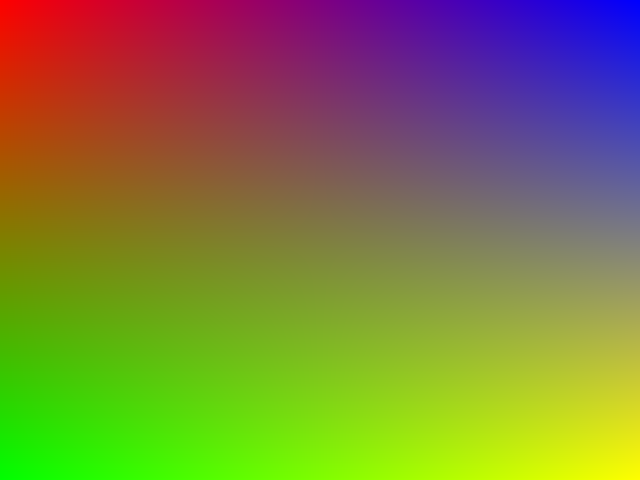
\includegraphics[width=150pt]{gradient.png}
\caption{Gradient produced by interpolation}
\end{figure}

\begin{figure}
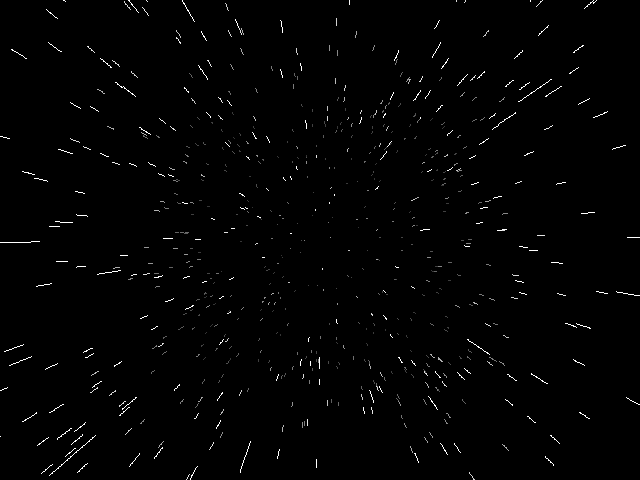
\includegraphics[width=150pt]{starfield.png}
\caption{Starfield with motion blur}
\end{figure}


\end{document}
